\documentclass{sig-alternate-05-2015}
\usepackage{paralist}
\usepackage{tikz}
\usepackage{float}
\usepackage{dblfloatfix}
\usepackage{graphicx}
\usepackage[font=small,labelfont=bf]{caption}
\usepackage{subcaption}
\usepackage{multirow}
\usepackage{balance}

%%%%%%%%%%%%%%%%%%%%%%%%%%%%%%%%%%%%%%%%%%%%%%%%%%%%%%%%%%%%%%%%%%%%%%%%%%%%%%%%
\begin{document} %%%%%%%%%%%%%%%%%%%%%%%%%%%%%%%%%%%%%%%%%%%%%%%%%%%%%%%%%%%%%%%

% Copyright
\setcopyright{acmcopyright}
\conferenceinfo{NOSSDAV '16}{May 10--13, 2016, Klagenfurt am W\"{o}rthersee,
  Austria}
%\doi{}
%\isbn{}
%\acmPrice{}

\title{Vertical Search Constraints in Multiview Motion Compensation}
\numberofauthors{1}
\author{
\alignauthor
Double-Blind Review
%Ben Hamlin, Wu-chi Feng\\
%       \affaddr{Portland State University}\\
%       \affaddr{Department of Computer Science}\\
%       \affaddr{P.O. Box 751}\\
%       \affaddr{Portland, OR 97207}\\
%       \email{<hamlinb> <wuchi>@cs.pdx.edu}
}

\maketitle

\begin{abstract}
Multiview video coding is an important technology for enabling streaming
stereoscopic video, among other applications. However, encoding multiple
views into one stream compounds the size and computation overhead of
traditional video coding. Because of this, there is a need to come up with new
ways to improve the space-time trade-off inherent in motion compensation
specialized for multiview. In this paper, we present and evaluate a simple
method to reduce the time-overhead of inter-view motion compensation by
constraining the search space vertically, leveraging knowledge of the
relationship between views. We show that this technique, which is
complementary to existing approaches, reduces the time taken by inter-view
motion compensation by a factor of two for views with one reference and a factor
of four for views with two references, with at most a small increase in
bit-rate. In addition, we provide an experimental analysis of view-dependency
structures in multiview video.
\end{abstract}

\begin{CCSXML}
<ccs2012>
<concept>
<concept_id>10002951.10003227.10003251</concept_id>
<concept_desc>Information systems~Multimedia information systems</concept_desc>
<concept_significance>500</concept_significance>
</concept>
</ccs2012>
\end{CCSXML}
\ccsdesc[500]{Information systems~Multimedia information systems}
\printccsdesc

\keywords{Video coding; motion compensation; multiview}

\section{Introduction} %%%%%%%%%%%%%%%%%%%%%%%%%%%%%%%%%%%%%%%%%%%%%%%%%%%%%%%%%
\label{sec:introduction} %%%%%%%%%%%%%%%%%%%%%%%%%%%%%%%%%%%%%%%%%%%%%%%%%%%%%%%
Multiview video coding (MVC) is a field that has emerged in the last two decades
to enable technologies such as stereoscopic video and free-viewpoint video. In
stereoscopic video, views from different, horizontally separated cameras are
presented to each eye to simulate a 3-dimensional scene. It is frequently useful
to have more than 2 views available to compensate for the viewer's distance from
the screen. Free-viewpoint video uses the views from multiple horizontally
separated cameras to allow the user to choose a vantage point on the scene. In
either case, it is necessary to encode at least two video streams together.

Multiview video presents bandwidth and storage challenges, since it is obviously
more expensive to transport or store multiple viewpoints than it is to transport
or store just one. Fortunately, since all the cameras are focused on the same
scene there is some inter-view redundancy, which can be taken advantage of such
that the combined views can be encoded more efficiently together than they could
be individually. The mechanism used to exploit inter-picture redundancy in
ITU/ISO H.264/MPEG4 AVC and Annex H, its multiview extension, is block-based
motion compensation. The most expensive aspect of this is motion-vector search,
and a variety of algorithms for it exist, many of which acheive impressive
results (a survey of existing algorithms is presented in \cite{khattak:fast}).

The novel approach we explore in this paper uses knowledge about the constrained
set of ways in which the pictures (in this case, the views) can differ from each
other in order to narrow down the possibilities before searching. Specifically,
in the common case for multiview, the cameras shooting the different views are
located in the same horizontal plane. This means that objects that are
non-occluded in both views will have different x-coordinates, but should not
have different y-coordinates. Thus we propose constraining the inter-view
motion-vector search to consider only horizontal motion-vector offsets, not
vertical ones.

Although the technique we propose is simple, it is an approach that has not, to
our knowledge, been examined in the literature, and it is not implemented in any
of the encoders we examined. Thus we feel that it is reasonable to ask whether
intuition -- that vertical constraint will reduce computation time without
significantly impacting quality or bit rate -- is borne out. We do so in this
paper, supporting our claim with experimental evidence. Our experiments produced
approximately a two-times speedup for views with one reference and about a
four-times speedup for views with two references, over using a fast search
algorithm alone, while incurring between $0\%$ and $7\%$ increase in bit-rate
depending on the content of the video.

The contributions of this work are twofold: \begin{compactitem}
\item We introduce the idea of vertical search constraints for inter-view
motion vectors and provide experimental data that demonstrates the kinds of
speedups and bit-rates it can achieve.
\item We present experimental data on the time taken and bit-rates achieved by a
variety of view-dependency structures, arriving at a suggestion for an optimal
8-view dependency structure and an intuition about in which cases unidirectional
and bidirectional inter-view dependencies are useful. \end{compactitem} To our
knowledge, this is the first paper to explore vertically constraining inter-view
motion compensation. For a summary of previous work on establishing optimal
view-dependency structures, the reader is refered to \cite{merkle:efficient}.

The remainder of this paper is organized as follows: In section
\ref{sec:algorithm} we discuss how we implemented vertical motion vector
constraint. We describe our results and the experimental methods we used to
obtain them in sections \ref{sec:results} and \ref{sec:method}, respectively.
Finally, in section \ref{sec:conclusion} we conclude the paper.

\section{Algorithm} %%%%%%%%%%%%%%%%%%%%%%%%%%%%%%%%%%%%%%%%%%%%%%%%%%%%%%%%%%%%
\label{sec:algorithm} %%%%%%%%%%%%%%%%%%%%%%%%%%%%%%%%%%%%%%%%%%%%%%%%%%%%%%%%%%
In this section, we describe our proposed technique for reducing the time taken
by inter-view motion compensation. In \ref{subsec:background} we describe motion
compensation and how it is used in the base H.264 standard and in MVC.
We restrict ourselves to discussing those aspects of inter-view motion
compensation that are relevant to the rest of our paper. For a more thorough
treatment of the advanced features of motion compensation in H.264 MVC, we
direct the reader to \cite{vetro:overview}. In \ref{subsec:constraining}, we
describe and motivate our technique for vertical search constraints.

\subsection{Motion Compensation}
\label{subsec:background}

Block-based motion compensation is a technique for reducing redundancies in two
pictures by encoding some or all of one with reference to the other. H.264 uses
a method similar to JPEG for encoding independent pictures. Pictures are divided
into blocks of varying sizes, each of which is transformed into the frequency
domain and stored as a set of coefficients to horizontally and vertically
oriented sinusoidal functions. These coefficients can then be quantized
to reduce the image's quality in ways that are difficult for the human eye to
perceive.

Once the block sizes have been chosen for a dependent picture, the reference
picture is searched for similar blocks of the same size at quarter-pixel
resolution. If two reference pictures are present, the encoder searches both
individually, then searches for pairs of blocks, one from each picture, that
produce a block similar to the dependent one when averaged. If a suitable block
is found, it is encoded as the spatial offset (in quarter-pixels) from the
dependent block to the reference block (a {\it motion vector}). The encoder then
takes the frequency-domain coefficient-wise difference between the two (the
{\it residual}) and encodes it along with the motion vector. The encoder may
also independently code blocks for which no match is found or {\it skip} blocks
that are identical to the reference picture.

Note that the standard does not specify how the search for motion vectors should
occur, only how the result should be encoded. Since it is generally the most
time-consuming part of the video coding process, encoders use a number of
methods to narrow down the search space. The first and most obvious is to limit
the search radius. Another approach (called {\it raster search}) is to reduce
the resolution of the search, so that only one block is searched per fixed-size
neighborhood. A third approach is to search in a fixed pattern (usually a
square, diamond, pentagon, hexagon, etc.) around a center point. The point
chosen becomes the new center, and the search is repeated with a decreased
radius, until at some point, the search finishes with a quarter-pixel full
search of some small area.

\subsection{Vertical Constraint} %%%%%%%%%%%%%%%%%%%%%%%%%%%%%%%%%%%%%%%%%%%%%%%
\label{subsec:constraining} %%%%%%%%%%%%%%%%%%%%%%%%%%%%%%%%%%%%%%%%%%%%%%%%%%%%

The above approaches assume that the best reference block is most likely to be
within a small area around the dependent block. This assumption is reasonable
in the case of motion compensation in the base H.264 standard, where reference
pictures are temporally offset by one or a few frames within the same video
stream ({\it inter} coding).

Stronger assertions can be made when using motion compensation to encode
temporally corresponding pictures within different views ({\it inter view}
coding). Assuming the views are being used for stereoscopic or free-viewpoint
video, objects shared between views always lie within the same horizontal plane.
In addition pictures from different views are always correlated. They are not
subject, for example, to being separated by scene changes. The only case in
which an object can be in one view but not in another is when it is occluded or
too skewed to be visually similar. It is this insight that leads us to propose
vertically constraining motion-vector search.

Our modifications to the encoding process are made quite simple by the fact that
practically every encoder already constrains the neighborhood in which motion
vectors are searched for. They typically specify a square around the original
block to search (e.g., $64\times 64$ pixels). Their search algorithm is usually
idenrical for inter and inter-view search. Our modification requires the encoder
to distinguish between the two types of motion compensation and, in the latter
case, reduce this neighborhood in the y-direction (e.g. to $64\times 1$ pixels).

Note that this is approach complementary to the existing techniques described in
in \ref{subsec:background}. Indeed, practically any search algorithm can be
vertically constrained, and the experimental evidence we present in
\ref{subsec:constrained} suggests that they would benefit from doing so, since
we are taking advantage of a property of the medium, not of a particular
algorithm. Additionally, our technique requires no modifications to be made in
the decoder, the player, or the standard, merely in the encoder.

\section{Experimental Method} %%%%%%%%%%%%%%%%%%%%%%%%%%%%%%%%%%%%%%%%%%%%%%%%%%
\label{sec:method} %%%%%%%%%%%%%%%%%%%%%%%%%%%%%%%%%%%%%%%%%%%%%%%%%%%%%%%%%%%%%
In this section, we describe the methods we used to obtain our results.
Subsections \ref{subsec:jmvc} and \ref{subsec:modifications} talk about the JMVC
reference codec and the modifications we made to it in order to obtain the data
we needed. Finally, in \ref{subsec:data-set} and \ref{subsec:environment}, we
talk about the data set we used and the hardware and software platform we ran
our tests on.

\subsection{Codec: JMVC}
\label{subsec:jmvc}
JMVC is the H.264 MVC reference codec \cite{schwarz:jmvc}. It is adapted from
JM \cite{suehring:jm}, the MPEG4/H.264 AVC reference codec, and contains a
complete implementation of the H.264 multiview extensions.

JMVC provides two methods of motion vector search: {\it block search}, which
tests every block in a region around the block being predicted for, and {\it
TZ-search}, which uses a combination of scaled-down raster search and diamond
refinement \cite{purnachand:improvements}. We ran tests using both algorithms,
but we will focus on our results using TZ-search, since this most closely
matches the way the codec is used in practice.

The codec also has several options when it comes to measuring the similarity
between blocks for motion compensation: sum of absolute differences (SAD); sum
of squared errors (SSE); or Hadamard. We used SAD for our tests, since it is
the simplest to reason about.

\subsection{Our Modifications}
\label{subsec:modifications}
In order to gather data about the coding process, we made the following changes
to the JMVC software: \begin{compactenum}
\item We instrumented the process of writing motion vectors to the byte-stream
by first writing the same information in human-readable format to a text file.
This allowed us to examine the motion vectors the codec produced and compare
them with the motion vectors we expected.
\item We inserted a timer around the process of encoding each picture, which
allowed us to determine exactly what portion of its time JMVC was spending on
each picture type.
\item We added a parameter to the configuration file that allowed us to
vertically constrain the motion-vector search space by a user-specified amount.
\end{compactenum}

In the process of making and testing these changes to JMVC, we discovered what
appears to be a bug in how it searches the reference picture for similar blocks.
The software allows the motion-vector search space to be limited to a square of
configurable size around the dependent block. In some cases, however, this
square goes off the edge of the picture and must be further restricted to end
at the picture's edges. In the case where the square went off the top or left
edge, JMVC did not properly constrain this square, resulting in the
motion-vector search going out of the bounds of the array the representing the
reference picture. The resulting garbage would occasionally yield a block that
the encoder found similar enough, resulting in motion vectors that referred to
blocks off the edge of the picture. We have reported this bug to the software's
maintainers.

\subsection{Data Set}
\label{subsec:data-set}
We ran our tests on 3D-rendered data-sets constructed specifically for testing
multi-view coding. We ran tests on two scenes: The first is of a bedroom, in
which the cameras pan horizontally across the room. The second depicts a
helicopter landing. See \cite{zhang:multi} for a description of the data set.

Despite being artificial, these scenes are representative of real multiview
scenes in that the views are rendered from different viewing angles such that
objects in one view may be occluded or skewed in adjacent views. Unlike
temporally separated pictures, different views cannot differ because of scene
changes, camera or object movement, etc. In principle, occlusion and skew are
the only causes of inter-view differences, and our data set adequately models
these.

Meanwhile, using constructed video streams, rather than the output of actual
multiview cameras, allows us to avoid artifacts that might occur in real
footage. For example, the cameras might be slightly tilted or out of horizontal
alignment, or one of the cameras might have a flawed lens. Although these are
considerations that come up in practice, our interest is in gathering data about
the common case, where the views have the expected correlation.

Each view contains 300 frames. Each frame is $1280\times 720$ pixels. Our tests
in \ref{subsec:optimal} and the full search in \ref{subsec:constrained} were run
using the first 100 frames from each data-set. The rest of our tests used all
300 frames.

We performed our timing tests for vertically constrained versus unconstrained
search using three view configurations. The first was the simplest configuration
possible: two views in which the first is the reference view, and the second
is dependent on the first. In addition to this, we ran tests on two eight-view
configurations. The structures of these and what motivated us to choose them
are described in \ref{subsec:optimal}.

\subsection{Testing Environment}
\label{subsec:environment}
All of our tests were performed on Red Hat Enterprise Linux version 4.1.2-54
using the SMP build of kernel version 2.6.18-371.6.1.el5. We encoded the YUV
files we used as input to JMVC using ffmpeg version 0.6.5. We compiled JMVC
with {\tt -O2} using gcc version 4.1.2. Our times were collected using GNU Time
version 1.7 for the per-view encoding times and {\tt clock\_gettime()} using
Linux's {\tt CLOCK\_MONOTONIC} for per-picture timing. Our hardware platforms
were servers with two hyper-threaded 4-core 2.4Ghz Intel Xeon processors. These
had cache sizes of 12288KB.

\section{Results} %%%%%%%%%%%%%%%%%%%%%%%%%%%%%%%%%%%%%%%%%%%%%%%%%%%%%%%%%%%%%%
\label{sec:results} %%%%%%%%%%%%%%%%%%%%%%%%%%%%%%%%%%%%%%%%%%%%%%%%%%%%%%%%%%%%
In this section, we present the results of our experiments. In
\ref{subsec:optimal} we motivate the view-dependency structures that we used
optimally in our experiments. In \ref{subsec:unconstrained} we analyze the
behavior of JMVC's motion compensation prior to our modifications. Lastly, in
\ref{subsec:constrained}, we show how applying vertical constraints improves
that behavior.

\subsection{Finding the Optimal View Structure}
\label{subsec:optimal}

\begin{figure}[h]
\centering
\begin{tabular}{|l|r|}
\hline
view type               & mean encoding time (seconds) \\
\hline
independent             & 465.13                       \\
dependent, 1 reference  & 348.99                       \\
dependent, 2 references & 1339.34                      \\
\hline
\end{tabular}
\caption{Time to encode 100 frames of each view type averaged over 10 trials
with each data-set.}
\label{fig:view-type-times}
\end{figure}

\begin{figure}[h]
\centering
\includegraphics[scale=.68]{figures/motion_vector_data_unconstrained_unidirectional.pdf}
\caption{
Average bit-rate for dependent view with one reference by distance from the
reference view.
}
\label{fig:uniframes}
\end{figure}

\begin{figure}[h]
\centering
\includegraphics[scale=.68]{figures/motion_vector_data_unconstrained_bidirectional.pdf}
\caption{
Average bit-rate for dependent view with two references by distance from the
reference views.
}
\label{fig:biframes}
\end{figure}

In order for us to reason about the effects of vertical search constraints, it
was necessary to decide upon a set of view structures to use. Since the
view dependencies could have an effect on the results of our experiments, it was
desirable to find the configuration with the optimal tradeoff between time and
bit-rate, on the assumption that it would be most likely to be used in
practice. We chose to run tests with two configurations: a simple two-view one,
and an eight-view one. In the case of a two-view configuration, the dependency
structure is obvious and allows for no optimization. It is not so obvious what
the optimal dependencies are when the number of views is increased to eight
however.

Since JMVC encodes at a variable bit-rate, there are two variables to optimize
for: bit-rate and time. Quality is fixed. Figure \ref{fig:view-type-times} shows
the average time taken to encode each view type, and Figures \ref{fig:uniframes}
and \ref{fig:biframes} show the average bit-rate of dependent pictures with one
and two references respectively, as a percentage of the bit-rate of
the average independent frame.

\begin{figure}[h]
\centering
\begin{subfigure}{.5\textwidth}
\centering
\resizebox{.8\textwidth}{!}{
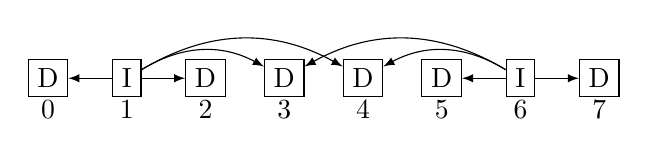
\begin{tikzpicture}[every path/.style={>=latex},every node/.style={draw,rectangle}]
\node            (a) at (0,0.4)  { D };
\node            (b) at (1,0.4)  { I };
\node            (c) at (2,0.4)  { D };
\node            (d) at (3,0.4)  { D };
\node            (e) at (4,0.4)  { D };
\node            (f) at (5,0.4)  { D };
\node            (g) at (6,0.4)  { I };
\node            (h) at (7,0.4)  { D };
\node[draw=none]     at (0,0)  { 0 };
\node[draw=none]     at (1,0)  { 1 };
\node[draw=none]     at (2,0)  { 2 };
\node[draw=none]     at (3,0)  { 3 };
\node[draw=none]     at (4,0)  { 4 };
\node[draw=none]     at (5,0)  { 5 };
\node[draw=none]     at (6,0)  { 6 };
\node[draw=none]     at (7,0)  { 7 };
\draw[->]             (b) edge (a);
\draw[->]             (b) edge (c);
\draw[->, bend left]  (b) edge (d);
\draw[->, bend right] (g) edge (d);
\draw[->]             (g) edge (h);
\draw[->]             (g) edge (f);
\draw[->, bend right] (g) edge (e);
\draw[->, bend left]  (b) edge (e);
\end{tikzpicture}}
\caption{
Optimal hierarchical configuration of \textbf{I}ndependent and
\textbf{D}ependent views.
}
\label{fig:hierarchical}
\end{subfigure} \\ \vspace{4pt}
\begin{subfigure}{.5\textwidth}
\centering
\resizebox{.8\textwidth}{!}{
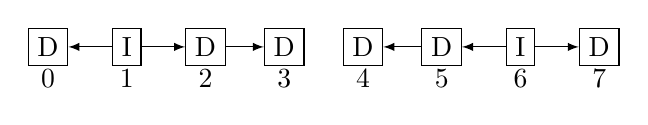
\begin{tikzpicture}[every path/.style={>=latex},every node/.style={draw,rectangle}]
\node            (a) at (0,0.4)  { D };
\node            (b) at (1,0.4)  { I };
\node            (c) at (2,0.4)  { D };
\node            (d) at (3,0.4)  { D };
\node            (e) at (4,0.4)  { D };
\node            (f) at (5,0.4)  { D };
\node            (g) at (6,0.4)  { I };
\node            (h) at (7,0.4)  { D };
\node[draw=none]     at (0,0)  { 0 };
\node[draw=none]     at (1,0)  { 1 };
\node[draw=none]     at (2,0)  { 2 };
\node[draw=none]     at (3,0)  { 3 };
\node[draw=none]     at (4,0)  { 4 };
\node[draw=none]     at (5,0)  { 5 };
\node[draw=none]     at (6,0)  { 6 };
\node[draw=none]     at (7,0)  { 7 };
\draw[->]             (b) edge (a);
\draw[->]             (b) edge (c);
\draw[->]             (c) edge (d);
\draw[->]             (g) edge (h);
\draw[->]             (g) edge (f);
\draw[->]             (f) edge (e);
\end{tikzpicture}}
\caption{
Optimal non-hierarchical configuration of \textbf{I}ndependent and
\textbf{D}ependent views.
}
\label{fig:non-hierarchical}
\end{subfigure}
\caption{Optimal eight-view dependency structures}
\label{fig:optimal}
\end{figure}

Although it is common practice to allow inter coding as well as inter-view
coding in dependent views, we have avoided this in our experiments in order
to isolate the effects of inter-view coding. Thus in our tests, an independent
view took slightly more time to encode than a dependent view with one reference,
because B-frames are much more time-consuming than P-frames. The most important
thing to note in Figure \ref{fig:view-type-times}, however, is that it takes
nearly four times as long to encode a view with two references than one with
one.

In Figure \ref{fig:biframes}, it's clear that frames with two references scale
more efficiently to the distance of their reference frames. Perhaps
surprisingly, however, a bidirectionally coded view with a distance of one from
either of its references has at most a very slightly better bit-rate than a
unidirectional view with a distance of one from its reference. Since it is
nearly four times as time-consuming, on average, to use two references, it is
hard to justify the meagre savings in bit-rate. Our vertical constraint
technique reduces the disparity between one- and two-reference views, making
dependent views with two references more viable.

Combining this information, we arrived at the two eight-view dependency
structures in Figure \ref{fig:optimal}. Figure \ref{fig:hierarchical} has the
smallest bit-rate possible with just two independent views, about 4.6$\times$
that of an independent view. On the other hand it is hierarchical, meaning that
if one wanted to send just two views (say, 1 and  6), one might need to send as
many as four reference views as well. The structure in
\ref{fig:non-hierarchical} takes care of this issue by having no hierarchical
dependencies. It has a bit-rate approximately 4.2$\times$ that of an independent
view.

\subsection{Distribution of Unconstrained \\ Motion Vectors}
\label{subsec:unconstrained}
In order to determine how well the existing motion-vector search was performing,
we modified JMVC to print out each of the motion vectors it produced for each of
our data sets. We then graphed those motion vectors' positions relative to the
dependent block to show how far afield the encoder was having to look for
satisfactory reference blocks.

\begin{figure}[h]
\centering
\begin{subfigure}{.5\textwidth}
\centering
\includegraphics[width=2.5in]{figures/helicopter-inter-mvs.pdf}
\caption{Independent}
\label{fig:inter-mvs}
\end{subfigure} \\
\begin{subfigure}{.5\textwidth}
\centering
\includegraphics[width=2.5in]{figures/helicopter-inter-view-mvs.pdf}
\caption{Dependent}
\label{fig:inter-view-mvs}
\end{subfigure}
\caption{
Independent and dependent view motion vectors from 2-view test of the helicopter
scene. Those from the bedroom scene are similar.
}
\label{fig:inter-and-inter-view-mvs}
\end{figure}

Figure \ref{fig:inter-mvs} shows the inter-coded motion vectors for the two-view
test. The motion vectors are clustered tightly around the location of the
dependent block.\footnote{The encoder has a bias toward motion vectors located
either directly above or below, or directly to the left or right of the origin.
This is due to the TZ-search algorithm, which searches in a diamond pattern, not
the content of the video.} In the inter-coded case, the motion vector search
does a good job of taking advantage of the temporal redundancy between
pictures. The inter-frame motion is small enough that a search centered at the
dependent block is able to quickly find appropriate motion vectors in most
cases, with very few motion vectors ending up distant from the origin.

Figure \ref{fig:inter-view-mvs} shows the motion vectors the unmodified JMVC
software produced for the dependent views of the same test. In contrast to the
inter-coded motion vectors, these are much more widely distributed, although
they tend to hug the x-axis. This can be attributed to two factors:
\begin{compactenum}
\item The ``right'' inter-view reference block according to the view
differential is farther away, horizontally, than is common for inter motion
vectors. This explains the increased horizontal spread.
\item The diamond refinement spends a lot of time looking at points off
the x-axis. Sometimes, it even finds a reference block that is ``good enough''
in a vertically offset position. This explains the increased vertical spread.
\end{compactenum} Note that the latter behavior is pathological: Except in the
case of occlusions and skew, {\it the best inter-view motion vector is always
horizontally, not vertically displaced.}

\begin{figure}[h]
\centering
\includegraphics[width=2.5in]{figures/helicopter-inter-view-bimvs1.pdf}
\caption{
Dependent view bidirectional motion vectors from 8-view test of the
helicopter data set.
}
\label{fig:inter-view-bimvs1}
\end{figure}

Figure \ref{fig:inter-view-bimvs1} shows similar data for two of the dependent
two-reference view of the non-hierarchical 8-view test. Again, there are a few
motion vectors that lie significantly off the x-axis, but by far the most
reflect the horizontal view offset. Notice that the motion vectors that lie on
the x-axis are centered farther from the origin than they are in
\ref{fig:inter-view-mvs}. This is consistent with the idea that they correspond
to view offset, in this case a greater offset than in \ref{fig:inter-view-mvs}.

\subsection{Benefits of Vertical Constraint}
\label{subsec:constrained}

\begin{figure}[h]
\centering\small
\begin{tabular}{|l|l|l|l|l|}
\multicolumn{1}{c}{} & \multicolumn{2}{c}{unconstrained} & \multicolumn{2}{c}{constrained} \\ \hline
algorithm            & bits            & secs.           & bits            & secs.         \\ \hline
full                 & 20935.92        & 142.58          & 22488.00        & 2.37          \\ \hline
TZ-search            & 21136.80        & 2.72            & 22551.12        & 1.43          \\ \hline
\end{tabular}
\caption{Seconds and bits per encoded frame of the dependent view of the
2-view test using full and TZ-search (100 frames).}
\label{fig:time-full-fast}
\end{figure}

Inspecting the dependent and reference blocks corresponding to motion vectors
that do not lie on the x-axis, we found that there are two primary reasons these
unexpected motion vectors occur: \begin{compactitem}
\item Some objects, such as the helicopter's shadow in the helicopter data set
as the camera zooms in, are visible in some views while not being visible in
others. Keeping view-dependencies adjacent minimizes this, but it still occurs.
In this case, allowing motion vectors that aren't on the x-axis can be useful,
since some other block might be a close-enough match.
\item Some blocks are general enough that they have close matches in many blocks
of the reference picture. For example, a section of bedroom wall looks very much
like every other section of bedroom wall. In this case, allowing motion vectors
off of the x-axis is probably not useful; even if the search algorithm happens
to find a vertically offset motion vector, it would likely be able to find one
with no vertical offset as well. \end{compactitem} Under the assumption that the
former case is relatively rare, we hypothesized that constraining the motion
vector search to the x-axis would have little effect on bit-rate.

\begin{figure}[h]
\centering
\begin{subfigure}{.5\textwidth}
\centering
\includegraphics[width=2.5in]{figures/bedroom1-inter-view-constrained-mvs.pdf}
\caption{Bedroom data set}
\label{fig:bedroom-inter-view-constrained-mvs}
\end{subfigure} \\
\begin{subfigure}{.5\textwidth}
\centering
\includegraphics[width=2.5in]{figures/helicopter-inter-view-constrained-mvs.pdf}
\caption{Helicopter data set}
\label{fig:helicopter-inter-view-constrained-mvs}
\end{subfigure}
\caption{Constrained unidirectional dependent view motion vectors from 2-view
test of each data-set.}
\label{fig:inter-view-constrained-mvs}
\end{figure}

Figure \ref{fig:time-full-fast} shows the time and bits required to encode each
frame using the full and TZ-search algorithms with and without vertical
constraint, and Figure \ref{fig:inter-view-constrained-mvs} shows the
distribution of the constrained motion vectors using TZ-search. Using the
vertical constraint produces shorter encoding times than using the TZ-search
alone, even when it is accompanied by the exhaustive full search algorithm.
Using vertical constraints and TZ-search together produces a speedup of
approximately $47\%$ over using TZ-search alone.

This speedup comes at the cost of a higher bit-rate, but only very slightly
-- in the case of the TZ-search, about a $6.7\%$ increase. This increase in
bit-rate is present even when the full search is used, which implies that these
blocks simply have no matching references on the x-axis. That is, it seems that
about $6$--$7\%$ of the blocks are occluded between these two adjacent views.

\begin{figure}[h]
\centering\small
\begin{subfigure}{.4\textwidth}
\centering
\begin{tabular}{|l|l|l|l|l|l|}
\multicolumn{2}{c}{} & \multicolumn{2}{c}{unconstrained} & \multicolumn{2}{c}{constrained} \\ \hline
view & num. refs.    & bits            & secs.           & bits            & secs.         \\ \hline
0    & 1             & 17503.73        & 2.74            & 17806.24        & 1.45          \\ \hline
2    & 1             & 18294.58        & 2.67            & 18751.60        & 1.44          \\ \hline
3    & 2             & 30397.04        & 11.88           & 30416.96        & 3.03          \\ \hline
4    & 2             & 30430.88        & 11.47           & 30398.82        & 2.93          \\ \hline
5    & 1             & 18661.41        & 2.62            & 19044.34        & 1.51          \\ \hline
7    & 1             & 19802.48        & 2.61            & 20109.01        & 1.48          \\ \hline
\end{tabular}
\caption{Bedroom data set}
\label{fig:bedroom-time-constrained}
\end{subfigure} \\
\begin{subfigure}{.4\textwidth}
\centering
\begin{tabular}{|l|l|l|l|l|l|}
\multicolumn{2}{c}{} & \multicolumn{2}{c}{unconstrained} & \multicolumn{2}{c}{constrained} \\ \hline
view & num. refs.    & bits            & secs.           & bits            & secs.         \\ \hline
0    & 1             & 35027.17        & 2.82            & 35299.28        & 1.34          \\ \hline
2    & 1             & 28179.97        & 2.68            & 28397.52        & 1.33          \\ \hline
3    & 2             & 47177.60        & 11.13           & 47287.41        & 2.64          \\ \hline
4    & 2             & 48463.14        & 11.32           & 48990.05        & 2.66          \\ \hline
5    & 1             & 30080.24        & 2.78            & 30688.85        & 1.34          \\ \hline
7    & 1             & 23016.29        & 2.66            & 23687.09        & 1.33          \\ \hline
\end{tabular}
\caption{Helicopter data set}
\label{fig:helicopter-time-constrained}
\end{subfigure}
\caption{Seconds and bits per encoded frame of the dependent views of the
non-hierarchical 8-view test. Views 1 and 6 (the independent views) are not
included, since we did not constrain the inter motion-vector search.}
\label{fig:time-constrained}
\end{figure}

Figure \ref{fig:time-constrained} contains the times and bit-rates required
to encode each frame of the dependent views of the 8-view hierarchical test.
Views 0, 2, 5, and 7 each have one reference, whereas views 3 and 4 each have
two. Figure \ref{fig:inter-view-constrained-bimvs1} shows the distribution of
motion vectors in view 3.

\begin{figure}[h]
\centering
\begin{subfigure}{.5\textwidth}
\centering
\includegraphics[width=2.5in]{figures/bedroom1-inter-view-constrained-bimvs1.pdf}
\caption{Bedroom data set}
\label{fig:bedroom-inter-view-constrained-bimvs1}
\end{subfigure} \hspace{4pt}
\begin{subfigure}{.5\textwidth}
\centering
\includegraphics[width=2.5in]{figures/helicopter-inter-view-constrained-bimvs1.pdf}
\caption{Helicopter data set}
\label{fig:helicopter-inter-view-constrained-bimvs1}
\end{subfigure}
\caption{Constrained bidirectional dependent view motion vectors from the view 3
of the hierarchical 8-view test.}
\label{fig:inter-view-constrained-bimvs1}
\end{figure}

For the one-reference views, speedups range from $42.3\%$ (bedroom, view 5) to
$52.4\%$ (helicopter, view 0). For the two-reference views, the
constrained version uniformly achieves speedups of about $75\%$. This large
decrease in the time taken to encode bidirectionally coded views serves to
make them more usable in practice: Without vertical constraints, a
two-reference view takes five times as long as a one reference view, and
probably isn't worth the cost in most cases. On the other hand, with vertical
constraints, they now take only twice as long, so the trade-off may be worth it.

The penalty in bit-rate varies, but in no case is it worse than than a
$2.9\%$ increase, and in most cases it is much less. In fact in one case
(bedroom, view 4), the bit-rate actually decreases in the constrained version.
This implies that whether and by how much the bit-rate will increase is highly
dependent on content.

\section{Conclusion} %%%%%%%%%%%%%%%%%%%%%%%%%%%%%%%%%%%%%%%%%%%%%%%%%%%%%%%%%%%
\label{sec:conclusion} %%%%%%%%%%%%%%%%%%%%%%%%%%%%%%%%%%%%%%%%%%%%%%%%%%%%%%%%%
This paper has two main goals: \begin{compactenum}
\item \label{itm:fst} To propose and examine the usefulness of vertical
constraints on inter-view motion-vector search; and
\item \label{itm:snd} To provide an experimental characterization of view
dependencies, with an eye toward arriving at an optimal dependency structure for
multiview video. \end{compactenum}

With respect to \ref{itm:fst}, using vertical constraints can provide
significant speedups with a small increase in bit-rate, due to occlusions. 
In particular, they provide about a four-times speedup for bidirectionally
coded views. The speedup they provide is large enough that this could be a
reasonable trade-off, especially for time-sensitive applications, like streaming
video.

With respect to \ref{itm:snd}, we have provided timing data for each view type,
averaged over several trials and two data sets, and bit-rate data for each
dependent view type, categorized by their distances from their reference views.
We demonstrated that bidirectionally coded views can scale more effectively to
view distance but come at a hefty cost in time. Fortunately, vertically
constraining inter-view motion vectors can drastically reduce the time they
take, making them more practical.

\balance
\bibliographystyle{abbrv}
\bibliography{bibliography}

\end{document} %%%%%%%%%%%%%%%%%%%%%%%%%%%%%%%%%%%%%%%%%%%%%%%%%%%%%%%%%%%%%%%%%
%%%%%%%%%%%%%%%%%%%%%%%%%%%%%%%%%%%%%%%%%%%%%%%%%%%%%%%%%%%%%%%%%%%%%%%%%%%%%%%%
